\documentclass[../main.tex]{subfiles}
\begin{document}

\section{Topological Equivariant Artist Model}
\label{sec:math}
To guide the implementation of structure preserving visualization components, we develop a mathematical formalism of visualization that specifies how these components preserve \textit{continuity} and \textit{equivariance}. Inspired by the analogous classes in Matplotlib\cite{hunterArchitectureOpenSource}, we call the transformation from data space to graphic space that these building block components implement the \textit{artist}.
\begin{equation}
    \label{eq:artist}
    \mathscr{\vartist}: \mathscr{\dtotal} \rightarrow \mathscr{\gtotal}
\end{equation}
The \textit{artist} $\mathscr{\vartist}$ is a map from data $\mathscr{\dtotal}$ to graphic $\mathscr{\gtotal}$ fiber bundles. To explain how the \textit{artist} is a structure preserving map from data to graphic, we first model data (\autoref{sec:math:data}) and graphics (\autoref{sec:math:graphic}) as topological structures that encapsulate component types and continuity. We then discuss the funtional maps from graphic to data (\autoref{sec:math:graphic:base}), data components to visual components (\autoref{sec:math:artist:nu}), and visual components into graphic (\autoref{sec:math:artist:q}) that make up the artist.

\subsection{Data Space \dtotal}
\label{sec:math:data}
We use fiber bundles as the data model because they are inclusive enough to express all the types of structures of data described in \autoref{sec:intro:data:tools}. A fiber bundle is a tuple $(\dtotal,\,\dbase,\,\pi ,\,\dfiber)$ defined by the projection map $\pi$
\begin{equation}
    \label{eq:fiber_bundle}
    \begin{tikzcd}
        \dfiber \arrow[r, hook] & \dtotal \arrow[r, "\pi"] & \dbase
    \end{tikzcd}
\end{equation}
that binds the components of the data in \dfiber\ to the continuity of the data encoded in \dbase. Our use of fiber bundles builds on Butler's work proposing that fiber bundles should be the common data abstraction for visualization data\cite{butlerVectorBundleClassesForm1992, butlerVisualizationModelBased1989}. The fiber bundle models the properties of data component types \dfiber\ (\autoref{sec:math:data:fiber}), the continuity of records \dbase\ (\autoref{sec:math:data:base}), the collections of records (\autoref{sec:math:data:section}), and the space \dtotal\ of all possible datasets with these components and continuity. By definition fiber bundles are locally trivial\cite{spanier1989algebraic,LocallyTrivialFibre}, meaning that over a localized neighborhood $U$ the total space is the cartesian product $\dbase\times\dfiber$. 

\subsubsection{Variables in Fiber Space \dfiber}
\label{sec:math:data:fiber}
To formalize the structure of the data components, we use Spivak's description of the schema \cite{spivakSIMPLICIALDATABASES} as a fiber bundle to bind the components of the fiber to variable names and data types. Spivak constructs a set \ftotal\ that is the disjoint union of all possible objects of types $\{\ftype_0, \ldots, \ftype_m\} \in \ftypes$, where \ftypes\ are the data types of the variables in the dataset. He then defines the single variable set \fttype\ 
\begin{equation}
    \label{eq:data_types}
    \begin{tikzcd}
        \fttype \arrow[r] \arrow[d, "\pi_{\fsection}"'] & \ftotal \arrow[d, "\pi"] \\
        \fnames \arrow[r, "\fsection"']                          & \ftypes       
    \end{tikzcd}
\end{equation}
which is \ftotal\ restricted to objects of type \ftype\ bound to variable name \fname. The \fttype\ lookup is by name to specify that every component is distinct, since multiple components can have the same type \ftype. Given \fsection, the fiber for a one variable dataset is
\begin{equation}
    \dfiber = \ftotal_{\fsection(\fname)} = \ftotal_{\ftype} 
\end{equation}
where \fsection\ is the schema that binds a variable name \fname\ to its datatype \ftype. A dataset with multiple components has a fiber that is the cartesian cross product of $\ftotal_{\fsection}$ applied to all the columns:
\begin{equation}
F = \ftotal_{\fsection(\fname_{1})}\times \ldots \ftotal_{\fsection(\fname_{i})} \ldots\times \ftotal_{\fsection(\fname_{n})}
\end{equation}
which can also be written as 
\begin{equation}
    \label{eq:math:data:fiber:decompose}
    \dfiber= \dfiber_{0} \times \ldots \times \dfiber_{i}\times\ldots\times \dfiber_{n}
\end{equation}
which allows us to decouple \dfiber\ into components $\dfiber_i = \ftotal_{\fsection{(\fname_{i})}}$.

\begin{figure}[H]
    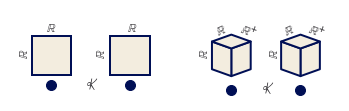
\includegraphics[width=1\textwidth]{figures/math/fiber.png}
    \caption{The fiber space is the cartesian product of the components.  The 2D fiber \(\dfiber=\reals\times\realsp\) (a) encodes the properties of \textit{time} and \textit{precipitation} components.  One dimension of the fiber encodes the range of possible values for the time component of the dataset, which is a subset of the \reals, while the other dimension encodes the range of possible values  \realsp\ for the precipitation component. This means the fiber is the set of points \textit{(precipitation, time)} that are all the combinations of \textit{precipitation} $\times$ \textit{time}. The 3D fiber (b) encodes points at all possible combinations of \textit{precipitation}, \textit{latitude}, and \textit{longitude}.}
    \label{fig:math:data:fiber}
\end{figure}

For example, the records in the 2D fiber (a) in \autoref{fig:math:data:fiber} are a pair of \textit{times} and \textit{precipitation} measurements taken at those times. Time is a positive number of type \texttt{datetime} which can be resolved to $\ftotal_{\texttt{datetime}}= \reals$. Precipitation values are real positive numbers $\ftotal_{\texttt{float}} = \realsp$. The fiber is 
\begin{equation*}
    \dfiber =  \reals \times \realsp 
\end{equation*} 
where the first component $F_0$ is the set of values specified by $(\fname=time,\, \ftype=\texttt{datetime},\, \fttype=\reals)$ and $F_1$ is specified by $(\fname=precipitation,\, \ftype=\texttt{float},\, \fttype=\reals)$ and is the set of values $\fttype=\reals$. In the 3D fiber (b) in \autoref{fig:math:data:fiber}, time is replaced with location. This location variable is of type \texttt{point} and has two components \textit{latitude} and \textit{longitude} $\{(lat,lon) \in \reals^{2} \mid  -90\leq lat \leq 90,\, 0 \leq lon \leq 360\}$. The fiber for this dataset is
\begin{equation*}
    \dfiber = \reals \times [0, 360] \times [-90, 90]
\end{equation*} 
and can either be thought of as having two components  
\begin{equation}
    \{(\fname=precipitation,\, \ftype=\texttt{float},\, \fttype=\reals), ((\fname = location,\, \ftype = \texttt{point},\, \fttype=\reals^{2})\}
\end{equation}
 or three
 \begin{equation}
    \{(\fname=precipitation,\, \ftype=\texttt{float},\, \fttype=\reals), (\fname=latitude,\, \ftype=\texttt{float}, \, \fttype=\reals), (\fname=longitude,\, \ftype=\texttt{float},\,\fttype=\reals)\}
 \end{equation}


\subsubsection{Measurement Scales: Monoid Actions}
\label{sec:math:data:monoid}
Implementing expressive visual encodings requires formally describing the structure on the components of the fiber, which we define by the actions of a monoid on the component. In doing so, we specify the properties of the component that must be preserved in a graphic representation. A monoid \cite{Monoid2021} $\monoid$ is a set with a binary operation $\ast:\monoid \times \monoid\rightarrow \monoid$ that satisfies the axioms:
\begin{align*}
    \textbf{associativity}\; & \text{for all} a, b, c \in \monoid \, (a \bullet b) \bullet c = a \bullet (b \bullet c)\\
    \textbf{identity}\; & \text{for all } a\in \monoid,\,  e\bullet a = a 
\end{align*} 
As defined on a component of \dfiber, a left monoid action \cite{SemigroupAction2021,nlab:action} of $\monoid_i$ is a set $\dfiber_i$ with an action $\bullet: \monoid\times \dfiber_i \rightarrow \dfiber_i$ with the properties:
\begin{align*}
    \textbf{associativity}\;& \text{for all } f,g \in \monoid_i \text{ and } x\in \dfiber_i,\, f\bullet(g\bullet x) = (f\ast g) \bullet x\\
    \textbf{identity}\;& \text{for all } x\in \dfiber_i, e\in \monoid_i,\,  e\bullet x = x 
\end{align*}
The identity and associativity properties of the action denote that the action is a monoid homomorphism, which means that the group operation is preserved on both sides of the action\cite{weissteinGroupHomomorphism}. 

\begin{figure}[H]
    \begin{subfigure}{.5\textwidth}
        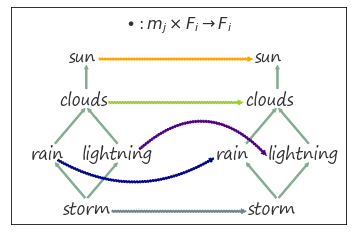
\includegraphics[width=\textwidth]{figures/math/monoid_total.png}
        \caption{}
        \label{fig:math:data:monoid:total}
    \end{subfigure}
    \begin{subfigure}{.5\textwidth}
        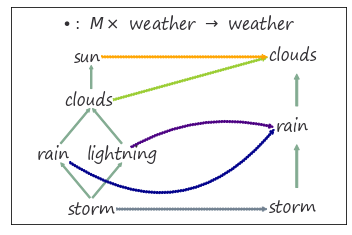
\includegraphics[width=1\textwidth]{figures/math/monoid_partial.png}
        \caption{}
        \label{fig:math:data:monoid:partial}
    \end{subfigure}
    \caption{The action $\bullet$ in \autoref{fig:monoid:total} is the arrows from the partial order diagram of weather states on the left to the diagram of weather states on the right. Since the action maps the weather states to themselves, the ordering defined by the monoid $\ast$ is preserved on both sides of the action. The action in \autoref{fig:monoid:partial} is monoid homomorphism because the ordering of the weather states is the same as the ordering of the elements they are mapped to. Given $sun \geq clouds\geq rain\, lightining$ on the right, the action  $sun\, clouds \rightarrow clouds$, and $rain\, lightining \rightarrow rain$ is structure preserving because on the left $cloud \geq rain$ so the relative ordering of elements is the same as the elements they are mapped to.}
    \label{fig:math:data:monoid}
\end{figure}

One example of monoids are partial orderings on a set, such as seen in \autoref{fig:math:data:monoid}. Each hasse diagram of the set of weather states describes an ordering on the set; the arrow goes from the lesser value to the greater one. For example, $storm \leq rain$. In \autoref{fig:monoid:total}, the action $\bullet$ maps the elements of a set of weather states into itself by mapping them into other elements of the weather states. The action in  \autoref{fig:math:data:monoid:total}, represented as the arrows between the hasse diagrams of the weather states, maps the weather states to themselves; therefore the ordering of the weather states is identical on both sides of the action and it is therefore homomorphic. The action $\bullet$ in \autoref{fig:math:data:monoid:partial} is a monotone map\cite{fongInvitationAppliedCategory2019}
\begin{equation*}
    if\, a \leq b \; then \; \bullet(a) \leq \bullet(b) \mid a,b \in \dfiber_{i}
\end{equation*}
where the structure the action preserves is the relative, rather than exact, ordering. Since groups are monoids with invertible operations, this definition of structure is also broad enough to include the Steven's measurment scales\cite{stevensTheoryScalesMeasurement1946,leaFormalizationMeasurementScale}. Monoids are also commonly found in functional programming since the core property of monoids is composability \cite{yorgeyMonoidsThemeVariations}. 

As with the fiber \dfiber\, the total monoid space \monoid\ is the cartesian product
\begin{equation}
    \label{eq:math:data:monoid:decompose}
\monoid= \monoid_{0} \times \ldots \times \monoid_{i}\times \ldots \times\ldots \monoid_{n}
\end{equation}
of each monoid $\monoid_{i}$ on $\dfiber_{i}$.  The monoid is also added to the specification of the fiber $(\fname_i,\, \ftype_i,\, \fttype\, \monoid_i)$

\subsubsection{Continuity of the Data $K$} 
\label{sec:math:data:base}
\begin{figure}[H]
    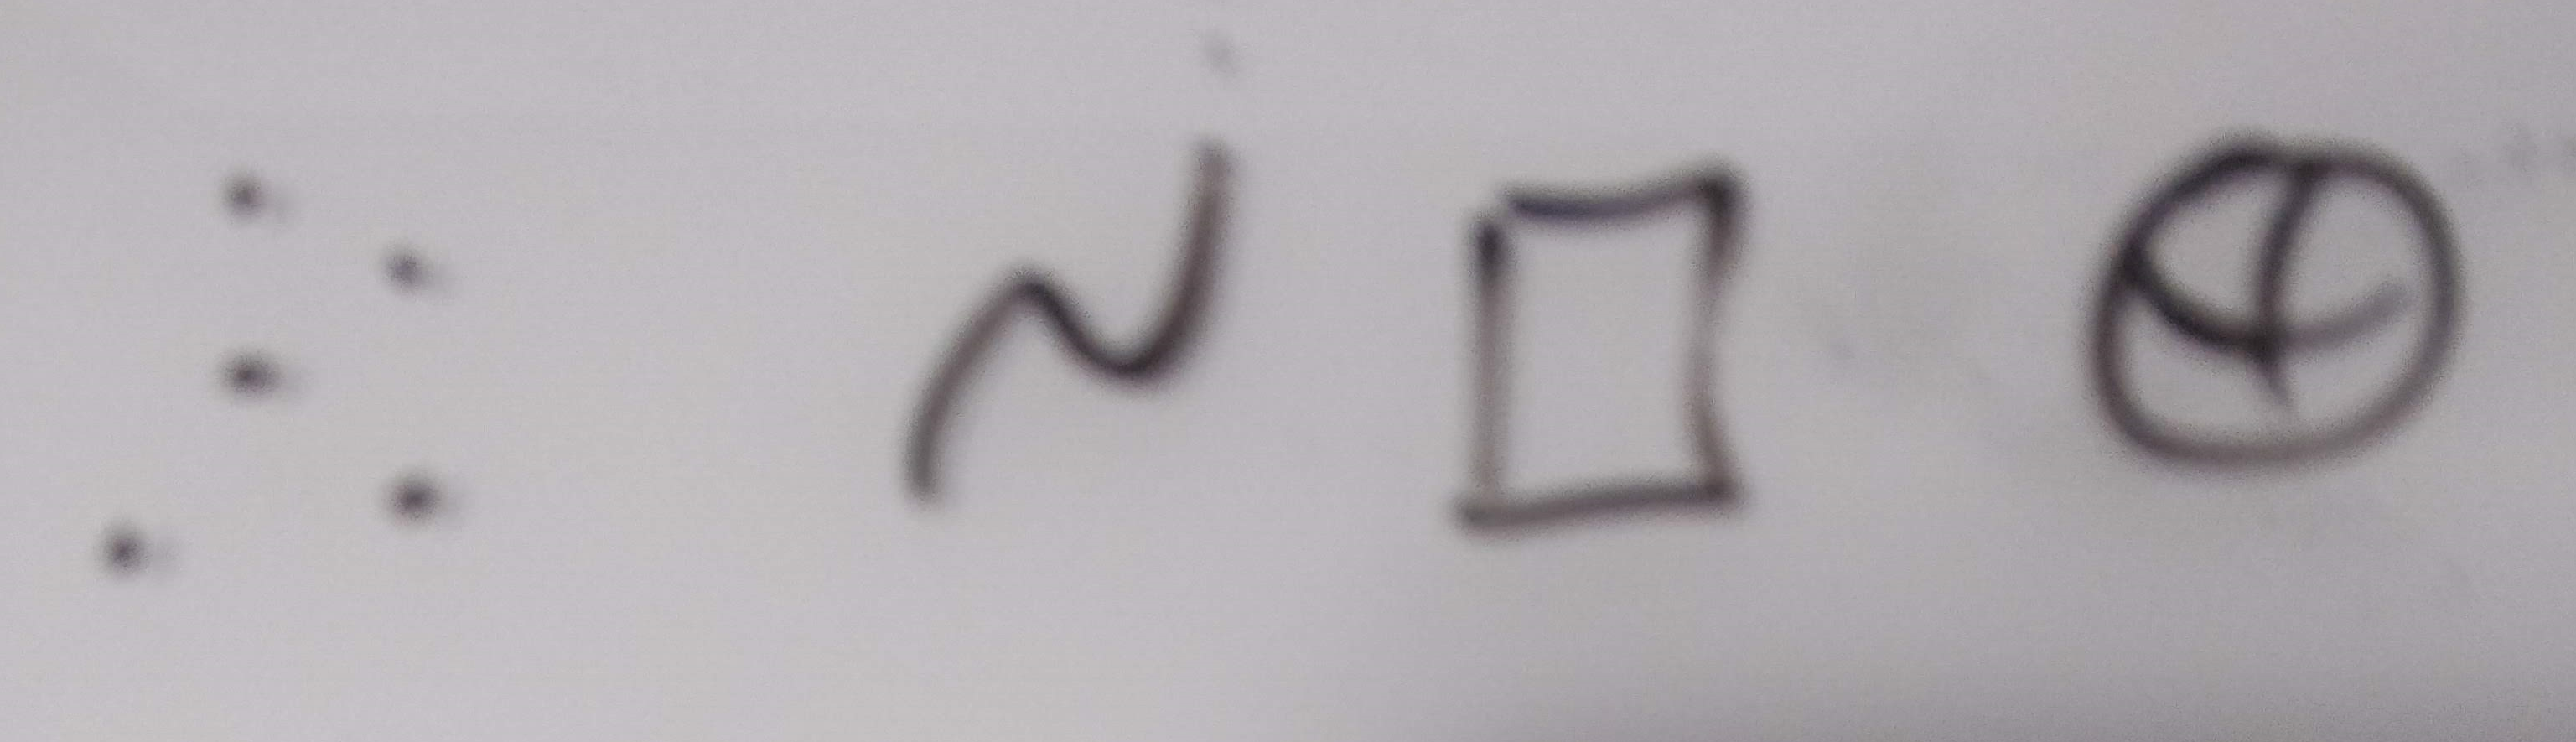
\includegraphics[width=1\textwidth]{figures/math/k_different_types.png}
    \caption{The topological base space \dbase\ encodes the continuity of the data space, for example if the data is discrete points or lies on a plane or a sphere}
    \label{fig:math:data:base:types}
\end{figure}
The base space \dbase\ acts as an indexing space, as emphasized by Butler\cite{butlerVectorBundleClassesForm1992,butlerVisualizationModelBased1989}, to express how the records in \dtotal\ are connected to each other. As shown in \autoref{fig:math:data:base:types}, 
\dbase\ can have any number of dimensions and can be continuous or discrete. The base space also does not describe anything about the dataset besides the continuity. While the base space may have components to identify the continuity, such as \textit{time, latitutde, longitude}, these labels are indexed into from \dbase\ the same as any other component. This is similar to the notion of structural \textit{keys} with associated \textit{values} proposed by Munzner\cite{munznerVisualizationAnalysisDesign2014}, but our model treats keys as a pure reference to topology. Decoupling the keys from their semantics allows the metadata to be altered; this provides for coordinate agnostic representation of the continuity and facilitates encoding of data where the independent variable may not be clear. For example the amount of snow on the ground is dependent on time of day and how much snow has fallen, and changing the coordinate system or time resolution should have no effect on how the records are connected to each other. 

\begin{figure}[H]
    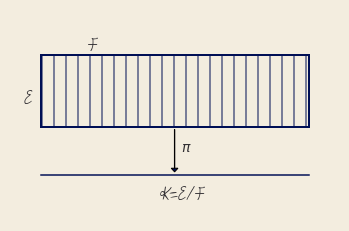
\includegraphics[width=\linewidth]{figures/math/k_qspace.png}
    \caption{The total space \dtotal\ is divided into fiber segments \dfiber. The base space \dbase\ acts as an index into the records in the fibers, such that every point \dbasepoint\ has a corresponding fiber $\dfiber_{\dbasepoint}$.}
    \label{fig:math:data:base:div}
\end{figure}

Formally \dbase\ is the quotient space \cite{QuotientSpaceTopology2020} of \dtotal\, meaning it is the finest space\cite{aurouxMath131Introduction} such that every $\dbasepoint \in \dbase$ has a corresponding fiber $\dfiber_k$\cite{QuotientSpaceTopology2020}. In \autoref{fig:math:data:base:div}, \dtotal\ is a rectangle divided by vertical fibers \dfiber, so the minimal \dbase\ for which there is always a mapping $\pi: \dtotal\rightarrow \dbase$ is the closed interval $\left[0,1\right]$. 

As with \autoref{eq:math:data:fiber:decompose} and \autoref{eq:math:data:monoid:decompose}, we can decompose the total space into component bundles $\pi:\dtotal_i\rightarrow \dbase$ where
\begin{equation}
    \label{eq:math:data:base:decompose}
    \pi:\dtotal_1\oplus\ldots\oplus \dtotal_i \oplus\ldots \oplus \dtotal_n \rightarrow \dbase
\end{equation}
such that \(\monoid_{i}\) acts on component bundle \(\dtotal_i\). The \dbase\ remains the same because the connectivity of records does not change just because there are fewer components in each record. By encoding this continuity in the model as \dbase\, the data model now explicitly carries information about its structure such that the implicit assumptions of the visualization algorithms are now explicit.
\begin{figure}[H]
    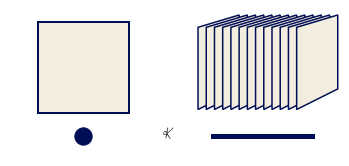
\includegraphics[width=1\textwidth]{figures/math/base.png}
    \caption{The fiber bundles in (a) and (b) encode the two component dataset from \autoref{fig:math:data:fiber}, with \textit{(time, precipitation)} components, as having different continuities. The fiber bundle with discrete continuity (a) encodes the dataset as being a set of discrete records. The fiber bundle over the continuous interval \dbase\ (b) encodes the records as if they were sampled from a 1D continuous space.} 
    \label{fig:math:data:base}
\end{figure}

The datasets in \autoref{fig:math:data:base} have the same fiber of (precipitation, time). The dot represents a discrete base space \dbase, meaning that every dataset encoded in the fiber bundle has discrete continuity. The line is a representation of a 1D continuity, meaning that every dataset in the fiber bundle is 1D continous. By encoding this continuity in the model as \dbase\, the data model now explicitly carries information about its structure such that the implicit assumptions of the visualization algorithms are now explicit. The explicit topology is a concise way of distinguishing visualizations that appear identical, for example heatmaps and images.  
 
\subsubsection{Data \dsection}
\label{sec:math:data:section}
While the projection function $\pi:\dtotal \rightarrow\dbase$ ties together the base space \dbase\ with the fiber \dfiber, a section $\dsection: \dbase\rightarrow \dtotal$ encodes a dataset. A section function takes as input location $\dbasepoint \in \dbase$ and returns a record $\delement \in \dtotal$. For example, in the special case of a table \cite{spivakSIMPLICIALDATABASES}, \dbase\ is a set of row ids, \dfiber\ is the columns, and the section \dsection\ returns the record \delement\ at a given key in \dbase. For any fiber bundle, there exists a map
\begin{equation}
    \begin{tikzcd}
        \dfiber \arrow[r, hook] & \dtotal \arrow[d, "\pi"'] \\
                          & \dbase \arrow[u, "\dsection"', bend right]
    \end{tikzcd}
\end{equation}
 such that $\pi(\dsection(\dbasepoint)) = \dbasepoint$. The set of all global sections is denoted as $\Gamma(\dtotal)$. Assuming a trivial fiber bundle $\dtotal = \dbase \times \dfiber$, the section is 
\begin{equation}
    \label{eq:section_return}
    \dsection(\dbasepoint) = (\dbasepoint, (g_{\dfiber_{0}}(\dbasepoint), \ldots, g_{\dfiber_{n}}(\dbasepoint)))
\end{equation}
where $g: \dbase \rightarrow \dfiber$ is the index function into the fiber. This formulation of the section also holds on locally trivial sections of a non-trivial fiber bundle. Because we can decompose the bundle and the fiber (\autoref{eq:math:data:base:decompose}, \autoref{eq:math:data:fiber:decompose}), we can decompose \dsection\ as 
\begin{equation}
\label{eq:math:data:section:decompose}
\dsection= (\dsection_0,\ldots, \dsection_i, \dots, \dsection_n) 
\end{equation}
where each section $\dsection_i$ maps into a record on a component $\dfiber_i \in \dfiber$. This allows for accessing the data component wise in addition to accessing the data in terms of its location over \dbase.

\begin{figure}[H]
    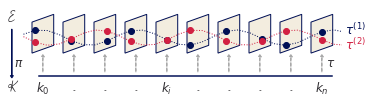
\includegraphics[width=1\linewidth]{figures/math/fiberbundle.png}
    \caption{ Fiber (time, precipitation) with an interval \dbase\ basespace. The sections $\dsection^{(1)}$ and $\dsection^{(2)}$ are constrained such that the time variable must be monotonic, which means each section is a timeseries of precipitation values. They are included in the global set of sections  $\dsection^{(1)}, \dsection^{(2)} \in \Gamma(\dtotal)$}
    \label{fig:math:data:sections}
\end{figure}

In \autoref{fig:math:data:sections}, the fiber is the same encoding of $(time, \, precipitation)$ illustrated in \autoref{fig:math:data:fiber}, and the base space is the interval \dbase\ shown in \autoref{fig:math:data:base}. The section $\dsection^{(1)}$ is a function that for a point \dbasepoint\ returns a record in the fiber \dfiber. The section applied to a set of points in \dbase\ resolves to a series of monotonically increasing in time records of \textit{(time, precipitation)} values. Section $\dsection^{(2)}$ returns a different timeseries of \textit{(time, precipitation)} values. Both sections are included in the global set of sections $\dsection^{(1)}, \dsection^{(2)} \in \Gamma(\dtotal)$.

\subsubsection{Sheafs}
\label{sec:math:data:sheaf}
Many types of dynamic visualizations require evaluating sections on different subspaces of \dbase, an a sheaf, denoted $\mathcal{O}$ provides a way to do so. A sheaf is a mathematical structure for defining collections of objects\cite{ghristElementaryAppliedTopology2014, ghristHomologicalAlgebraData2018,urbanikBriefIntroductionSchemes} on mathematical spaces. On the fiber bundle \dtotal, we can describe a sheaf as the collection of local sections $\iota^{*}\dsection$
\begin{equation}
    \label{eq:sheaf}
    \begin{tikzcd}[column sep=huge]
        \iota^*\dtotal \arrow[d, "\pi"'] \arrow[r, "\iota^*", hook]             & \dtotal \arrow[d, "\pi"']                  \\
        U \arrow[r, "\iota", hook] \arrow[u, "\iota^{*}\dsection"', bend right] & \dbase \arrow[u, "\dsection"', bend right]
    \end{tikzcd}
\end{equation}
which are sections of \dtotal\ pulled back over local neighborhood $U \subset \dtotal$ via the inclusion map \(\iota:\dtotal\rightarrow U\). The collation of sections enabled by sheafs is necessary for navigation techniques such as pan and zoom\cite{NekrasovskiEvaluationPanZoom2006} and dynamically updated visualizations such as sliding windows\cite{crouchDynamicGraphsSlidingwindow2013,chuTimeSeriesSegmentation1995}.

\subsubsection{Applications to Data Containers}
This model provides a common formalism for widely used data containers without sacrificing the semantic structure embedded in each container. For example, the section can be any instance of a univariate numpy array\cite{harris2020array} that stores an image.  This could be a section of a fiber bundle where \dbase\ is a 2D continuous plane and the \dfiber\ is $(\reals^{3}, \reals, \reals)$ where $\reals^3$ is color, and the other two components are the x and y positions of the sampled data in the image. This position information is already implicitely encoded in the array as the index and the resolution of the image being stored.Instead of an image, the numpy array could also store a 2D discrete table. The fiber would not change, but the \dbase\ would now be 0D discrete points. These different choices in topology indicate, for example, what sorts of interpolation would be appropriate when visualizing the data. 

There are also many types of labeled containers that can richly be described in this framework because of the schema like structure of the fiber. For example, a pandas series which stores a labeled list, or a dataframe\cite{jeff_reback_2020_3715232} which stores a relational table. A series could store the values of $\dsection^{(1)}$ and a second series could be  $\dsection^{(2)}$. We could also fatten the fiber to hold two precipitationure series, such that a section would be an instance of a dataframe with a time column and two precipitation columns. While the series and dataframe explicitly have a time index column, they are components in our model and the index is assumed to be data independent references such as hashvalues, virtual memory locations, or random number keys.

Where this model particularly shines are N dimensional labeled data structures. For example, an xarray\cite{hoyer2017xarray} data that stores precipitation field could have a \dbase\ that is a continuous volume and the components would be the precipitation and the time, latitude, and longitude the measurements were sampled at. A section can also be an instance of a distributed data container, such as a dask array \cite{rocklinDaskParallelComputation2015}. As with the other containers, \dbase\ and \dfiber\ are defined in terms of the index and dtypes of the components of the array. Because our framework is defined in terms of the fiber, continuity, and sections, rather than the exact values of the data, our model does not need to know what the exact values are until the renderer needs to fill in the image.  

\subsection{Graphic Space \gtotal}
\label{sec:math:graphic} 
To establish that the artist is a structure preserving map from data \dtotal\ to graphic \gtotal\, we construct a graphic bundle so that we can define \textit{equivariance} in terms of maps on the fiber spaces and \textit{continuity} in terms of maps on the base space. As with the data, we can represent the target graphic as a section \gsection\ of a bundle  $(\gtotal, \gbase, \pi, \gfiber)$. 
\begin{equation}
    \begin{tikzcd}[ampersand replacement=\&]
        \gfiber \arrow[r, hook] \& \gtotal \arrow[d, "\pi"'] \\
                          \& \gbase \arrow[u, "\gsection"', bend right]
    \end{tikzcd}
  \end{equation}
The graphic bundle \gtotal\ consists of a base \gbase (\autoref{sec:math:graphic:fiber}) that is a thickened form of \dbase\, a fiber \gfiber (\autoref{sec:math:graphic:base}) that is an idealized display space, and sections \gsection (\autoref{sec:math:graphic:section}) that encode a graphic where the visual characteristics are fully specified.

\subsubsection{Idealized Display \gfiber}
\label{sec:math:graphic:fiber}
To fully specify the visual characteristics of the image, we construct a fiber \gfiber\ that is a non-pixelated version of the target space. Typically \gtotal\ is trivial and therefore sections can be thought of as mappings into \gfiber. In this work, we assume a 2D opaque image $\gfiber=\reals^5$ with elements 
\begin{equation*}
(x,\, y,\, r,\, g,\, b) \in \gfiber
\end{equation*}
such that a rendered graphic only consists of 2D position and color. To support overplotting and transparency, the fiber could be $\gfiber=\reals^{7}$ such that $(x, y, z, r, g, b, a) \in \gfiber$ specifies the target display. By abstracting the target display space as \gfiber, the model can support different targets, such as a 2D screen or 3D printer. 

\subsubsection{Continuity of the Graphic \gbase} 
\label{sec:math:graphic:base}
\begin{figure}[H]
    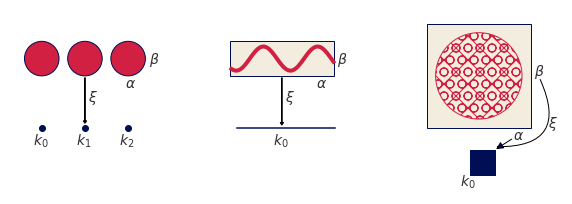
\includegraphics[width=1\textwidth]{figures/math/retraction_maps.png}
    \caption{For a visualization component to preserve continuity, it must have a continuous surjective map $\vindex: \gbase\rightarrow\dbase$ from graphic continuity to data continuity. The scatter (a) and line (b) graphic base spaces \gbase\ have one more dimension of continuity than \dbase\ so that \gbase\ can encode physical aspects of the glyph, such as shape (a circle) or thickness. The image (c) has the same dimension in \gbase\ as in \dbase\ because \dbase\ is already 2D and therefore can directly map into screen space.}
    \label{fig:math:graphic:retraction:map}
\end{figure}
To establish that a visualization component preserves continuity, we propose that their must be a continuous map $\vindex: \gbase\rightarrow\dbase$ from the graphic base space to the data space. For example, consider a \gbase\ that is mapped to the region of a 2D display space that represents \dbase. For some visualizations, \dbase\ may be lower dimension than \gbase. For example, a point that is 0D in \dbase\ cannot be represented on screen unless it is thickened to 2D to encode the connectivity of the pixels that visually represent the point. This thickening is often not necessary when the dimensionality of \dbase\ matches the dimensionality of the target space, for example if \dbase\ is 2D and the display is a 2D screen. We introduce \gbase\ to thicken \dbase\ in a way which preserves the structure of \dbase. 

Formally, we require that \dbase\ be a deformation retract\cite{RetractionTopology2020} of \gbase\ so that \dbase\ and \gbase\ have the same homotopy, meaning there is a continuous map from \gbase\ to \dbase\cite{weissteinHomotopy}. The surjective map $\vindex: \gbase \rightarrow \dbase$ 
\begin{equation}
    \begin{tikzcd}
        \dtotal \arrow[d, "\pi"'] & \gtotal \arrow[d, "\pi"'] \\
        \dbase                   & \gbase \arrow[l, "\vindex"']
    \end{tikzcd}
    \label{eq:math:graphic:vindex}
\end{equation}
goes from region $\gbasepoint \in \gbase_{\dbasepoint}$ to its associated point $\gbasepoint$. This means that if $\vindex(\gbasepoint) = \dbasepoint$, the record at \dbasepoint\ is copied over the region \gbasepoint\ such that $\dsection(\dbasepoint)=\vindex^*\dsection(\gbasepoint)$ where $\vindex^*\dsection(\gbasepoint)$  is \dsection\ pulled back over \gbase. The map \vindex\ is part of the implementation of the artist $\mathcal{\vartist}$ and therefore is not defined in terms of the data; instead it is how we specify the constraint that the type of the graphic \textit{continuity} must be able to map to the type of the data \textit{continuity}. When \dbase\ is discrete points and the graphic is a scatter plot, each point $\dbasepoint \in \dbase$ can correspond to a 2D disk $\gbase_{\dbasepoint}$ as shown in \autoref{fig:math:graphic:retraction:map}. In the case of 1D continuous data and a line plot, the region \gy\ over a point $\gx_i$ specifies the thickness of the line in \gbase\ for the corresponding \dsection\ on \dbasepoint. The image has the same dimensions in data space and graphic space such that no extra dimensions are needed in \gbase. 

The mapping function \vindex\ provides a way to identify the part of the visual transformation that is specific to the the connectivity of the data rather than the values; for example it is common to flip a matrix when displaying an image. The \vindex\ mapping is also used by interactive visualization components to look up the data associated with a region on screen.  One example is to fill in details in a hover tooltip, another is to convert region selection (such as zooming) on \gbase\ to a query on the data to access the corresponding record components on \dbase.

\subsubsection{Graphic \gsection}
\label{sec:graphic_section}
The section $\gsection: \gbase \rightarrow \gtotal$ is the graphic in an idealizes prerender space and also acts as a specification for rendering the graphic to an image. It is sufficient to sketch out how an arbitrary pixel would be rendered, where a pixel $p$ in a real display corresponds to a region $\gbase_p$ in the idealized display. To determine the color of the pixel, we aggregate the color values over the region via integration:
\begin{align*}
    \label{eq:math:graphic:section:color}
    r_p &= \iint\limits_{S_p} \rho_r(s)ds^{2}\\
    g_p &= \iint\limits_{S_p} \rho_g(s)ds^{2}\\
    b_p &= \iint\limits_{S_p} \rho_b(s)ds^{2}
\end{align*}
For a 2D screen, the pixel is defined as a region $p=\left[y_{top}, y_{bottom}, x_{right}, x_{left}\right]$ of the rendered graphic. Since the x and y in $p$ are in the same coordinate system as the x and y components of \gfiber\,  the inverse map of the bounding box $\gbase_{p} ={\gsection_{xy}}^{-1}(p)$ is a region $\gbase_p \subset \gbase$. The color is the result of the integration over  $\gbase_p$.

\begin{figure}[H]
    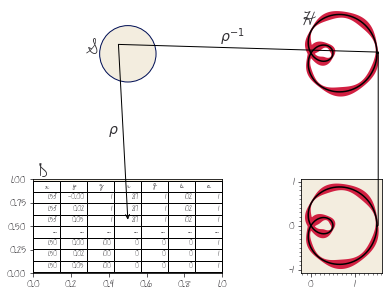
\includegraphics[width=\textwidth]{figures/math/render.png}
    \caption{To render a graphic, a pixel $p$ is selected in the display space, which is defined in the same coordinates as the x and y components in \gfiber\ via the renderer. In \gtotal\, the inverse mapping ${\gsection_{xy}}^(p)$ returns a region $\gbase_{p} \subset \gbase$. $\gsection(\gbase_{p})$ returns a set of points $(x,\,y,\,r,\,g,\,b) \in \gfiber$ that lie over $\gbase_{p}$. The integral over the $(r,\,g,\,b)$ pixels specifies that the pixel should be green}
    \label{fig:math:graphic:rho:lookup}
\end{figure}

As shown in \autoref{fig:math:graphic:rho:lookup}, a pixel $p$ in the output space, drawn in yellow, is selected and mapped, via the renderer, into a region on \gtotal.  The region on \gtotal\ corresponds to a region $\gbase_p \subset \gbase$ via the inverse mapping  ${\gsection_{xy}}^(p)$. The base space \gbase\ is an annulus to match the topology of the graphic idealized in \gtotal. The section  $\gsection(\gbase_{p})$  then maps into the fiber \gfiber\ over $\gbase_p$ to obtain the set of points in \gfiber, here represented as a table, that correspond to that section. The integral over the pixel components of this set of points in the fiber yields \{3, 135, 60\} the actual color of the pixel. In general, \gsection\ is an abstraction of rendering. In very broad strokes \gsection\  can be a specification such as PDF\cite{bienz1993portable}, SVG\cite{quintScalable2003}, or an openGL scene graph\cite{CarsonOpenGL1997}. Alternatively, \gsection\ can be a rendering engine such as cairo\cite{CairographicsOrg} or AGG\cite{shemanarevAntiGrainGeometry}. Implementation of \gsection\ is out of scope for this work,

\subsection{Artist}
\label{sec:artist}
The topological artist \vartist\ is how we model the building block component that transforms data into a graphic. The artist \vartist\ is a map from the sheaf on a data bundle \dtotal\ which is $\mathcal{O}(\dtotal)$ to the sheaf on the graphic bundle \gtotal, $\mathcal{O}(\gtotal)$. 
\begin{equation}
    \vartist: \mathcal{O}(\dtotal) \rightarrow \mathcal{O}(\gtotal)
    \label{eq:math:artist:artist}
\end{equation}
The artist preserves \textit{continuity} through the \vindex\ map discussed in \autoref{sec:math:graphic:base}. We conjecture that it is an \textit{equivariant} map because it carries a homomorphism of monoid actions \cite{cegarraCohomologyMonoidsOperators2019}
\begin{equation}
    \varphi: \monoid \rightarrow \monoid^{\prime}
\end{equation}

Given \monoid\ on data $\mathscr{\dtotal}$ and $\monoid^{\prime}$ on graphic $\mathscr{\gtotal}$, we propose that artists $\mathscr{\vartist}$ are equivariant maps 
\begin{equation}
\vartist(m\cdot \delement) = \varphi(m)\cdot \vartist(\delement) 
\end{equation}
such that applying a monoid action $m \in \monoid$ to the data input $\delement \in \mathscr{\dtotal}$ of the artist $\mathscr{\vartist}$ is equivalent to applying a monoid action $\varphi(\monoid) \in \monoid^{\prime}$ to the graphic $\vartist(\delement) \in \mathscr{\gtotal}$ output of the artist.

The monoid equivariant map has two stages: the encoders $\vchannel:\dtotal^{\prime} \rightarrow \vtotal$ convert the data components to visual components, and the assembly function $\vmark: \vtotalpull \rightarrow \gtotal$ composites the fiber components of \vtotalpull\ into a graphic in \gtotal.
\begin{equation}
    \label{eq:math:artist:diagram}
    \begin{tikzcd}
        \dtotal \arrow[r, "\vchannel"] \arrow[rd, "\pi"'] & \vtotal \arrow[d, "\pi"] & \vindex^*\vtotal \arrow[r, "\vmark"] \arrow[d, "\vindex^*\pi"'] \arrow[l, "\vindex^*"'] & \gtotal \arrow[ld, "\pi"] \\
                                              & \dbase                  & \gbase \arrow[l, "\vindex"']                                              &                    
        \end{tikzcd}
\end{equation}
\vtotalpull\ is the visual bundle \vtotal\ pulled back over \gbase\ via the equivariant continuity map $\vindex:\gbase \rightarrow \dbase$ introduced in \autoref{sec:math:graphic:base}.
The functional decomposition of the visualization artist in \autoref{eq:math:artist:diagram}facilitates building reusable components at each stage of the transformation because the equivariance constraints are defined on \vchannel, \vmark, and \vindex. We name this map the artist as that is the analogous part of the  Matplotlib\cite{hunterArchitectureOpenSource} architecture that builds visual elements.

\subsubsection {Visual Fiber Bundle \vtotal}
\label{sec:math:visual}
We introduce a visual bundle \vtotal\ to store the mappings of the data components into components of the graphic. The visual bundle $(\vtotal,\,\dbase,\,\pi ,\,\vfiber)$ is the space of possible parameters of a visualization type, such as a scatter or line plot. As with the data and graphic bundles, the visual bundle is defined by the projection map $\pi$
\begin{equation}
    \begin{tikzcd}[ampersand replacement=\&]
        \vfiber \arrow[r, hook] \& \vtotal \arrow[d, "\pi"'] \\
                          \& \dbase \arrow[u, "\vsection"', bend right]
    \end{tikzcd}
\end{equation}
where \vsection\ is the visual variable encoding, as described by Bertin \cite{bertinSemiologyGraphicsDiagrams2011a}, of the data section \dsection. The visual fiber \vfiber\ is defined in terms of the input parameters of the visualization library's plotting functions; by making these parameters explicit components of the fiber, we can build consistent definitions and expectations of how these parameters behave.
\begin{table}[H]
    \centering
    \renewcommand{\arraystretch}{2}
    \begin{tabulary}{\textwidth}{|l|L|l|}\hline
     $\bm{\vchannel_{i}}$                      & $\bm{\vsection_{i}}$                                                            & $\bm{codomain(\vchannel_{i}) \subset \vfiber_{i}}$  \\ \hline                                              
    position                    & x, y, z, theta, r                                                          & $\mathbb{R}$   \\ \hline
    size                        & linewidth, markersize                                            & $\mathbb{R}^{+}$   \\ \hline
    shape                       & markerstyle                                                      & $\{f_{0}, \ldots, f_{n}\}$ \\ \hline
    color                       & color, facecolor, markerfacecolor, edgecolor  & $\mathbb{R}^{4}$ \\ \hline
    \multirow{2}{*}{texture}    & hatch                                                            & $\mathbb{N}^{10}$\\\cline{2-3}
                                & linestyle                                                        & $(\mathbb{R}, \mathbb{R^+}^{n, n\%2=0})$ \\ \hline              
    \end{tabulary}
    \caption{Some possible components of the fiber \vfiber\ for a visualization function implemented in Matplotlib}
    \label{tab:math:artist:mpl:fiber}
\end{table}
 A section \vsection\ is a tuple of visual values that specifies the visual characteristics of a part of the graphic. For example, given a fiber of \(\{x, y, color\}\) one possible section could be  \(\{.5, .5, (255, 20,147)\}\). The \(codomain(\vchannel_i)\) determines which monoids can act on $\vfiber_i$. These fiber components are implicit in the library, as seen in \autoref{tab:math:artist:mpl:fiber}, and by making them explicit as components of the fiber we can build consistent definitions and expectations of how these parameters behave. 

 
\subsubsection{Visual Encoders \vchannel}
\label{sec:math:artist:nu}
We define the visual transformers \vchannel\ 
\begin{equation}
  \label{eq:math:artist:nu}
  \{\vchannel_{0}, \ldots, \vchannel_{n}\}: \{\dsection_{0}, \ldots, \dsection_{n}\} \mapsto \{\vsection_{0}, \ldots, \vsection_{n}\}
\end{equation}
as the set of equivariant maps $\vchannel_i: \dsection_i \mapsto \vsection_i$. Given $\monoid_i$ is the monoid action on $\dtotal_i$ and that there is a monoid ${\monoid_i}^{\prime}$ on $\vtotal_i$, then there is a monoid homomorphism from $\varphi:\monoid_i \rightarrow {\monoid_i}^{\prime}$ that \vchannel\ must preserve. As mentioned in \autoref{sec:math:data:monoid}, monoid actions define the structure on the fiber components and are therefore the basis for equivariance. A validly constructed \vchannel\ is one where the diagram of the monoid transform $m$ commutes
\begin{equation}
  \label{eq:math:artist:nu_commute}
\begin{tikzcd}
  \dtotal_i \arrow[r] \arrow[r, "\vchannel_i"] \arrow[d, "m_{\delement}"'] & \vtotal_i \arrow[d, "m_{\velement}"] \\
  \dtotal_i \arrow[r, "\vchannel_i"]                           & \vtotal_i               
\end{tikzcd}
\end{equation}
such that applying equivariant monoid actions to $\dtotal_{i}$ and $\vtotal_{i}$ preserves the map $\vchannel_{i}: \dtotal_{i}\rightarrow \vtotal_{i}$. In general, the data fiber $\dfiber_{i}$ cannot be assumed to be of the same type as the visual fiber $\vfiber_{i}$ and the actions of \monoid\ on $\dfiber_{i}$ cannot be assumed to be the same as the actions of $\monoid^{\prime}$ on \vfiber; therefore an equivariant $\vchannel_i$ must satisfy the constraint  
\begin{equation}
\vchannel_i(m_{\delement}(\dtotal_i)) = \varphi(m_{\delement})(\vchannel_i(\dtotal_i))
\label{eq:math:artist:nu:equivariance}
\end{equation} 
such that $\varphi$ maps a monoid action on data to a monoid action on visual elements. However, we can construct a monoid action of \monoid\ on $\vfiber_{i}$ that is compatible with a monoid action of \monoid\ on $\dfiber_{i}$. We can compose the monoid actions on the visual fiber $\monoid^{\prime} \times \vfiber_{i} \rightarrow \vfiber_{i}$ with the homomorphism $\varphi$ that takes \monoid\ to $\monoid^{\prime}$. This allows us to define a monoid action on \vfiber\ of \monoid\ that is $(m, \velement) \rightarrow \varphi(m)\bullet\velement$. Therefore, without a loss of generality, we can assume that an action of \monoid\ acts on $\dfiber_{i}$ and on $\vfiber_{i}$ compatibly such that $\varphi$ is the identity function. 

\begin{figure}[htb]
  \centering
  \begin{subfigure}{.49\textwidth}
    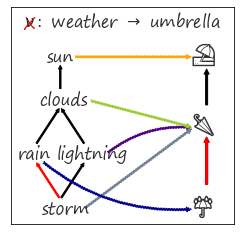
\includegraphics[width=1\textwidth]{figures/math/partial_invalid.png}
    \caption{}
    \label{fig:math:artist:nu:invalid}
  \end{subfigure}
  \begin{subfigure}{.49\textwidth}
    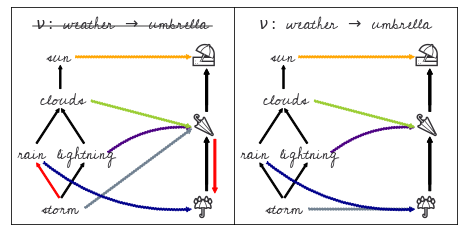
\includegraphics[width=1\textwidth]{figures/math/partial_fixed.png}
    \caption{}
    \label{fig:math:artist:nu:valid}
  \end{subfigure}
  \caption{The map from data component to visual component in \autoref{fig:math:artist:nu:invalid} is not homomorphic, and therefore invalid, because $rain \geq storm$ is mapped to elements with the reverse ordering $\nu(storm) \geq \nu(storm)$. In contrast, the mapping in \autoref{fig:math:artist:nu:valid} is valud since $\nu(storm)=\nu(rain)$ satisfies the condition $\nu(storm) \geq \nu(storm)$}
  \label{fig:math:artist:nu}
\end{figure}

The translation from weather state data to visual representation as umbrella emoji in \autoref{fig:math:artist:nu:invalid} is an invalid visual encoding map \vchannel\ because it is not homomorphic. This is because the monotonic condition \(rain \geq storm \implies \vchannel(rain) \geq  \vchannel(storm)\) is not met since \(\vchannel(rain) \leq\vchannel(storm)\). To satisfy the monotonic condition for $rain \geq storm$, either red arrow in \autoref{fig:math:artist:nu:invalid} would have to go in a different direction. On the other hand, the mapping from weather state to umbrellla in \autoref{fig:math:artist:nu:valid} is a homomorphism since $\vchannel(rain) = \vchannel(storm)$ satisfies the monotonic condition of $rain \geq storm$. \autoref{fig:math:artist:nu} is an example of how the model supports partially ordered data components, which was a motivation for defining equivariance as monoid homomorphisms. 

\begin{table}[H]
\centering
  \renewcommand{\arraystretch}{2}
  \begin{tabulary}{\columnwidth}{|llL|}\hline
      \textbf{scale} & \textbf{group} & \textbf{constraint}\\ \hline
      nominal & permutation &  $\text{if } \delement_1 \neq \delement_2 \text{ then } \vchannel (\delement_1) \neq\vchannel(\delement_2)$\\
      ordinal &  monotonic & $\text{if } \delement_1 \leq \delement_2 \text{ then } \vchannel (\delement_1) \leq \vchannel(\delement_2)$\\
      interval &  translation &  $\vchannel (x + c) = \vchannel(x) + c$ \\
      ratio &  scaling &  $\vchannel(xc) = \vchannel(x)*c $\\ \hline
  \end{tabulary}
  \caption{}
  \label{tab:math:artist:nu}
\end{table}

The Stevens measurement types\cite{stevensTheoryScalesMeasurement1946}, listed in \autoref{tab:math:artist:nu}, are specified in terms of groups, which are monoids with invertible operations\cite{remlingAlgebraMath5353}. Despite critiques of the scales\cite{johnsonPseudoMathematicsMentalSocial1936,thomasMathematizationNotMeasurement2014}, we believe it is critical for the model to include the measurement scales since they are commonly used in visualization to classify components \cite{munznerVisualizationAnalysisDesign2014,wilkinsonGrammarGraphics2005}. By specifying the equivariance constraints on \vchannel\, we can guarantee that the stage of the artist that transforms data components into visual representations is equivariant. These constraints guide the implementation of reusable component transformers \vchannel\ that are composed when generating the graphic. 


\subsubsection{Visualization Assembly}
\label{sec:math:artist:q}
\begin{figure}[htb]
  \centering
  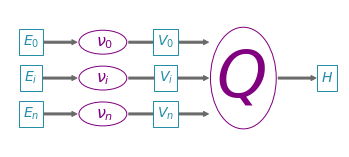
\includegraphics[width=\textwidth]{figures/math/path_of_q.png}
  \caption{The transform functions $\vchannel_i$ convert data $\dsection_i\in \dtotal$ to visual characteristics $\vsection_i \in \vtotal$, then \vmark\ assembles $\vsection_i$ into a graphic $\gsection \in \gtotal$.} 
  \label{fig:math:artist:q}
\end{figure}
The transformation from data into graphic is analagous to a map-reduce operation; as illustrated in \autoref{fig:math:artist}, data components $\dtotal_{i}$ are mapped into visual components $\vtotal_{i}$ that are reduced into a graphic in \gtotal. The space of all graphics that \vmark\ can generate is the subset of graphics reachable via applying the reduction function $\vmark(\Gamma(\vtotal)) \in \Gamma(\gtotal)$ to the visual section $\vsection \in \Gamma(\vtotal)$. The full space of graphics is not necessarily equivariant; therefore we formalize the constraints on \vmark\ such that it produces structure preserving graphics. 

We formalize the expectation that visualization generation functions parameterized in the same way should generate the same functions as the equivariant map $\vmark: \vsection \mapsto \gsection$. We then define the constraint on \vmark\ such that if \vmark\ is applied to two visual sections $\vsection$ and $\vsection^{\prime}$ that generate the same \gsection\, then the output of $\vsection$ and $\vsection^{\prime}$ acted on by the same monoid $m$ must be the same.  We do not define monoid actions on all of $\Gamma(\gtotal)$ because there may be graphics $\gsection \in \Gamma(\gtotal)$ for which we cannot construct a valid mapping from \vtotal.
\begin{figure}[htb]
  \centering
  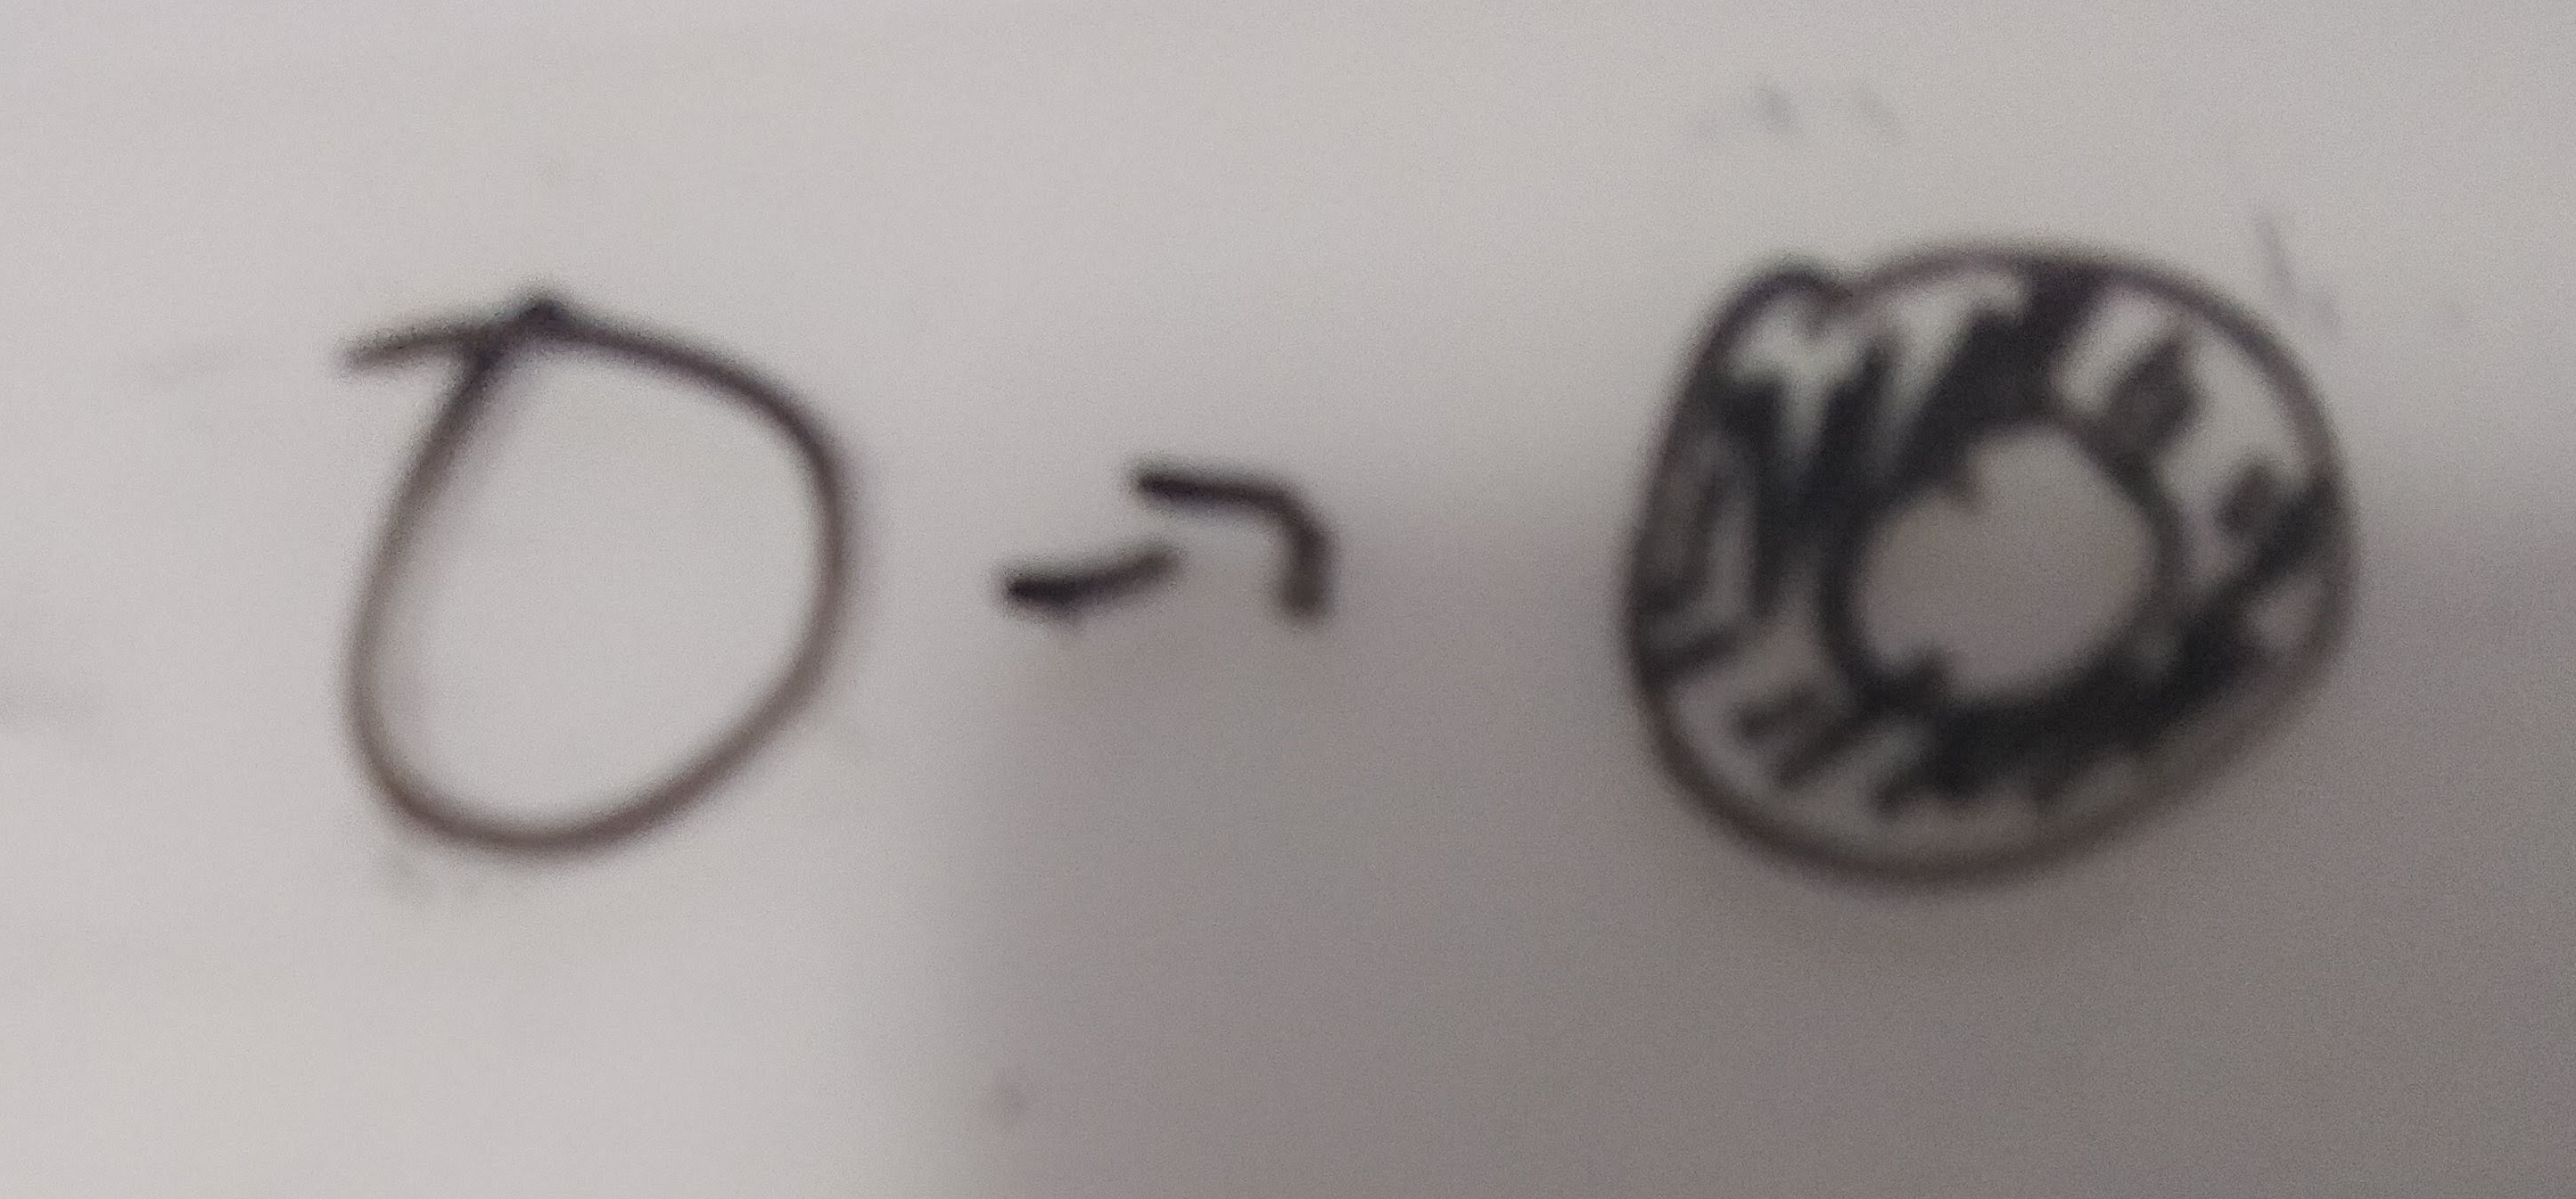
\includegraphics[width=\textwidth]{figures/math/diff_type_q.png}
  \caption{These two glyphs are generated by the same annulus \vmark\ function. The monoid action $m_i$ on edge thickness $\vsection_i$ of the first glyph yields the thicker edge ${\vsection_i}^{\prime}$ in the second glyph.}
  \label{fig:math:artist:graphic}
\end{figure}
Lets call the visual representations of the components $\Gamma(\vtotal)=X$ and the graphic $\vmark(\Gamma(\vtotal))=Y$
\begin{prop}
If for elements of the monoid $m \in \monoid$ and for all $\vsection, \vsection^{\prime} \in X$, we define the monoid action on $X$ so that it is by definition equivariant
\begin{equation}
\vmark(\vsection) = \vmark(\vsection^{\prime})\implies \vmark(m\circ\vsection) = \vmark(m\circ\vsection^{\prime})
\label{eq:math:artist:q}
\end{equation}
then a monoid action on $Y$ can be defined as $m\circ \gsection = \gsection^{\prime}$. If and only if \vmark\ satistfies \autoref{eq:math:artist:q}, we can state that the transformed graphic $\gsection^{\prime}=\vmark(m\circ \vsection)$ is equivariant to a monoid action applied on \vmark\ with input $\vsection \in \vmark^{-1}(\gsection)$ that must generate valid \gsection. 
\end{prop}

For example, given fiber $\vfiber=(xpos,\, ypos,\, color,\, thickness)$, then sections $\vsection=(0,0,0,1)$ and $\vmark(\vsection) = \gsection$ generates a piece of the thin hollow circle. The action $m=(e, e, e, x+2)$, where e is identity, translates \vsection\ to  $\vsection^{\prime}=(e,e,e,3)$ and the corresponding action on \gsection\ causes $\vmark(\vsection^{\prime})$ to be the thicker circle in \autoref{fig:math:artist:graphic}.

We formally describe a glyph as \vmark\ applied to the regions \dbasepoint\ that map back to a set of path connected components $\dbasepath \subset \dbase$ as input 
\begin{equation}
\dbasepath = \{\dbasepathpoint \in \dbase \text{ s. t. } \exists \gamma \text{ s.t. } \gamma(0)=\dbasepoint \text{ and }\gamma(1)=\dbasepathpoint\}
\end{equation}
where the path\cite{ConnectedSpace2020}  $\gamma$ from \dbasepoint\ to \dbasepathpoint\ is a continuous function from the interval [0,1]. We define the glyph as the graphic generated by $\vmark(\gbase_{\dbasepathpoint})$
\begin{equation}
  \begin{tikzcd}
      \gtotal \arrow[r, shift left] & \gbase_\dbasepathpoint \arrow[rr, "\vindex(\gbasepoint)", shift left] \arrow[l, "\gsection(\gbase_\dbasepathpoint)"] &  & \dbasepath_{\dbasepoint} \arrow[ll, "\vindex^{-1}(\dbasepath)"]
      \end{tikzcd}
  \label{eq:mark}
\end{equation}
such that for every glyph there is at least one corresponding region on \dbase, in keeping with the definition of glyph as any visually differentiable element put forth by Ziemkiewicz and Kosara\cite{ziemkiewiczEmbeddingInformationVisualization2009}. The primitive point, line, and area marks\cite{bertinSemiologyGraphicsDiagrams2011a,carpendaleVisualRepresentationSemiology} are specially cased glyphs.
  

\subsubsection{Assembly \vmark}
Given the continuities described in \ref{fig:math:graphic:retraction:map}, 
we illustrate a minimal Q that will generate the most minimal visualizations associated with those continuities: non-overlapping scatter points, a non-infinitely thin line, and an image. 
\begin{figure}[H]
    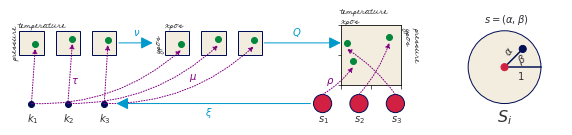
\includegraphics[width=1\textwidth]{figures/math/scatter_with_s.png}
    \caption{The data is discrete points (precipitation, time). Via \vchannel\ these are converted to (xpos, ypos) and pulled over discrete \gbase. These values are then used to parameterize \gsection\ which returns a color based on the parameters (xpos,ypos) and position $\alpha, \beta$ on $\gbase_{\dbasepoint}$ that \gsection\ is evaluated on. 
    }
    \label{fig:math:artist:q:scatter}
\end{figure}
The scatter plot in \autoref{fig:math:artist:q:scatter} has a constant size and color $\gsection_{RGB} = (0,0,0)$ that are defined as part of the point assembly function.

\begin{figure} [H]

\begin{minipage}{.5\textwidth}
    \begingroup \leqnomode
    \begin{equation}
        \vmark(xpos, ypos)(\alpha, \beta)
        \label{eq:eq:math:artist:q:scatter}
    \end{equation}
    \endgroup
    \begin{align*}
        x &= \text{size} *\alpha \cos(\beta) + xpos \\[.5\baselineskip]
        y &= \text{size} *\alpha \sin(\beta) + ypos
    \end{align*}
\end{minipage}
\begin{minipage}{.5\textwidth}
    \centering
    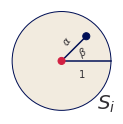
\includegraphics{figures/math/scatter_s.png}
\end{minipage}
\caption{The simplest form of the scatter plot takes as input the expected position of the marker in visual space \textit{(xpos, ypos)}. The marker shape is determined by the polar coordinates $(\alpha, \beta)$ on the disc; these coordinates dictate whether anything is drawn at that region of \gbase. To obtain the color of the pixel at \textit{(x,y)}, the region on \gbase\ is scaled by a constant size and shifted by the \textit{xpos} and \textit{ypos}.}
\label{fig:math:artist:q:scatter:s}
\end{figure}
The position of this swatch of color is computed relative to the location on the disc \((\alpha, \beta) \in \gbase_{\dbasepoint}\) as shown in \autoref{fig:math:artist:q:scatter:s}. The region $\alpha, \beta)$ is scaled by a constant size and shifted by \textit{xpos} and \textit{ypos}. This computation yields the values \textit{(x,y)} that map into \gfiber\ and have a corresponding function $\gsection(\gbasepoint) = (x, y, 0, 0, 0)$ which colors the point \textit{(x,y)} black. 

\begin{figure}[H]
    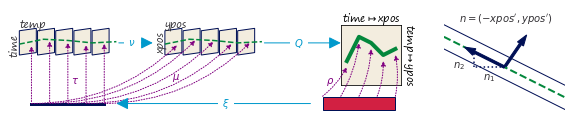
\includegraphics[width=\textwidth]{figures/math/line_with_s.png}
    \caption{The line fiber $(time,\, temp)$ is thickened with the derivative $(time^{\prime},\, precipitation^{\prime}$ because that information will be necessary to figure out the tangent to the point to draw a line. This is because the line needs to be pushed perpendicular to the tangent of (xpos, ypos). The data is converted to visual characteristics (xpos, ypos). The $\alpha$ coordinates on \gbase\ specifies the position of the line, the $\beta$ coordinate specifies thickness.}
    \label{fig:math:artist:q:line}
\end{figure}
In contrast, the line plot in \autoref{fig:math:artist:q:line} has a \vindex\ function that is not only parameterized on \dbasepoint\ but also on the $\alpha$ distance along \dbasepoint\ and corresponding region in \gbase. 

\begin{figure} [H]
    \begin{minipage}{.5\textwidth}
        \begingroup \leqnomode
        \begin{equation}
            \vmark(xpos, n_1, ypos, n_2 )(\alpha, \beta) 
            \label{eq:eq:math:artist:q:line}
        \end{equation} \endgroup
        \begin{align*}
            \lvert n \rvert &=\sqrt{{n_{1}}^2(\vindex(\alpha)) + {n_{2}}^2(\vindex(\alpha))} \\
            \hat{n}_{1} &= \frac{n_1(\vindex(\alpha))}{\lvert n \rvert}, \,\hat{n}_{2} = \frac{n_2(\vindex(\alpha))}{\lvert n \rvert} \\[.5\baselineskip]
            x &= xpos(\vindex(\alpha)) + \text{width}*\beta\hat{n}_1(\vindex(\alpha))  \\
            y &= ypos(\vindex(\alpha)) + \text{width}*\beta\hat{n}_2(\vindex(\alpha)) 
           \end{align*}
    \end{minipage}
    \begin{minipage}{.5\textwidth}
        \centering
        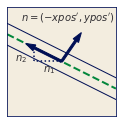
\includegraphics{figures/math/line_s.png}
    \end{minipage}
    \caption{The \textit{xpos} and \textit{ypos} variables give the position of the line in screen space, but render an infinitely thin line. To draw equidistant lines parallel to(\textit{xpos}, \textit{ypos}), defined by the distance  $(n_1, n_2)$, requires the derivatives $(n_{1} = xpos^{\prime}, n_{2} = ypos^{\prime})$. The position (\textit{xpos}, \textit{ypos}) and width of the line is then used to determine whether a pixel is colored at the position (\textit{x}, \textit{y}). The values in data space are only looked up via the $\alpha$ coordinate of \gbase\ because it maps to a location on \dbase. The $\beta$ parameter is used to specify how thick the line is in conjunction with the constant width. }
    \label{fig:math:artist:q:line:s}
\end{figure}
As shown in \autoref{fig:math:artist:q:line:s}, line needs to know the tangent of the data to draw an envelope above and below each (xpos,ypos) such that the line appears to have a thickness; therefore the artist takes as input the jet bundle \cite{JetBundle2020,musilovaCalculusVariationsJet2016} $\mathcal{J}^{2}(\dtotal)$ which is the data \dtotal\ and the first and second derivatives of \dtotal. The indexing map $\vindex(\alpha)$ finds the point in \dbase\ corresponding to the region in \gbase\ at coordinate $\alpha$. The section \dsection\ on the \dbasepoint\ that corresponds to the region in \gbase\ returns the position \textit{xpos, ypos} and the derivatives $\hat{n}_1, \hat{n}_2$ . The derivatives are then multiplied by a width parameter to specify the thickness of the line. This is then used to determine the color of the pixel at \textit{(x,y)}.  

\begin{figure}[H]
    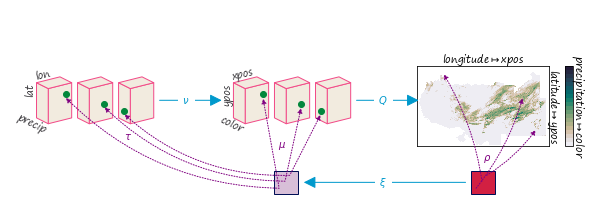
\includegraphics[width=\textwidth]{figures/math/image.png}
    \caption{Via \vindex\, the artist maps from a point \textit{(x,y)} on the screen to a corresponding point on \dbase. This maps into \dfiber\ via \dsection. These data points are converted to visual points via \vchannel\, and then \vmark\ assembles the \textit{(xpos, ypos, color)} parameters into attributes of each pixel. }
    \label{fig:math:artist:q:heatmap}
\end{figure}
In \autoref{fig:math:artist:q:heatmap}, the image is a direct lookup into  $\vindex:\gbase\rightarrow\dbase$. The indexing variables $(\alpha, \beta)$ define the distance along the space, which is then used by \vindex\ to map into \dbase\ to lookup the color values.
\begin{equation}
    \vmark(xpos, ypos, color)(\alpha, \beta)
    \label{eq:math:artist:q:image}
    \end{equation}
\begin{align*}
x &= xpos(\vindex(\alpha))\\
y &= ypos(\vindex(\beta))\\
R, G, B &= color(\vindex(\alpha, \beta))
\end{align*}
In the case of an image, the indexing mapper \vindex\ may do some translating to a convention expected by \vmark, for example reorientng the array such that the first row in the data is at the bottom of the graphic. 


\subsubsection{ \vmarkd}
\label{sec:math:artist:qhat}

\begin{figure}[htb]
    \centering
      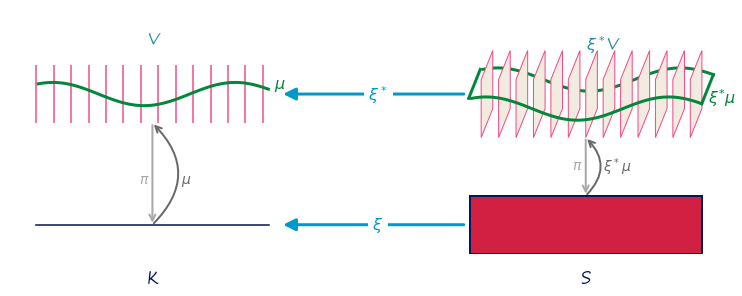
\includegraphics[width=1\textwidth]{figures/math/q_hat.png}
      \caption{Because the pullback of the visual bundle \vtotalpull\ is the replication of a \vsection\ over all points \gbasepoint\ that map back to a single \dbasepoint, we can constract a \vmarkd\ on \vsection\ over \dbasepoint\ that will fabricate the \vmark\ for the equivalent region of \gbasepoint\ associated to that \dbasepoint}
      \label{fig:math:artist:qhat}
  \end{figure}
  
The graphic base space \gbase\ is not accessible in many architectures, including Matplotlib; instead we can construct a factory function \vmarkd\ over \dbase\ that can build a \vmark. As shown in \autoref{eq:math:artist:diagram}, \vmark\ is a bundle map $\vmark: \vtotalpull\rightarrow \gtotal$ where \vtotalpull\ and \gtotal\ are both bundles over \gbase.
%[column sep=huge]
\begin{equation}
    \begin{tikzcd}
        \textcolor{gray!50}{\dtotal} \arrow[r, "\vchannel", color=gray!50] \arrow[rd, "\pi"', color=gray!50] & \vtotal \arrow[d, "\pi"']                  & \vindex^*\vtotal \arrow[r, "\vmark", color=gray!50] \arrow[d, "\vindex^*\pi"'] \arrow[l,  "\vindex^*"'] & \textcolor{gray!50}{\gtotal} \arrow[ld, "\pi", color=gray!50] \\
                                                          & \dbase \arrow[u, "\vsection"', bend right] & \gbase \arrow[l, "\vindex"'] \arrow[u, "\vindex^*\vsection"', bend right]               &                          
        \end{tikzcd}
        \label{eq:math:artist:qhat}
\end{equation}
The preimage of the continuity map $\vpreimg \subset \gbase$ is such that many graphic continuity points $\gbasepoint \in \gbase_{\dbase}$ go to one data continuity point \dbasepoint; therefore, by definition the pull back of \vsection\
\begin{equation}
    \vtotalpull \mid_{\vpreimg} = \vpreimg \times \vfiber
\end{equation}
copies the visual fiber \vfiber\ over the the points \gbasepoint\ in graphic space \gbase\ that correspond to one \dbasepoint\ in data space \dbase. This set of points \gbasepoint\ are the preimage \vpreimg\ of \dbasepoint. 

As shown in \autoref{fig:math:artist:qhat}, given the section \vsectionpull\ pulled back from \vsection\ and the point $\gbasepoint \in \vpreimg$, there is a direct map $(\dbasepoint, \vsection(\dbasepoint)) \mapsto (\gbasepoint, \vsectionpull(\gbasepoint))$  from \vsection\ over \dbasepoint\ to the section \vsectionpull\ over \gbasepoint. This means that the pulled back section $\vsectionpull(\gbasepoint) = \vindex^*(\vsection(\dbasepoint))$ is the section \vsection\ copied over all \gbasepoint such that \vsectionpull\ is identical for all \gbasepoint\ where $\vindex(\gbasepoint) = \dbasepoint$. In \autoref{fig:math:artist:qhat} each dot on \vfiber\ is equivalent to the line on \vfiberpull. 

Given the equivalence between \vsection\ and \vsectionpull\ defined above, the reliance on \gbase\ can be factored out. When \vmark\ maps visual sections into graphics $\vmark: \Gamma(\vtotalpull) \rightarrow \Gamma(\gtotal)$, if we restrict \vmark\ input to \vsectionpull\ then the graphic section \gsection\ evaluated on a visual region \gbasepoint\
\begin{equation}
    \gsection(\gbasepoint) \coloneqq \vmark(\vsectionpull)(s)
    \label{eq:math:artist:qhat}
\end{equation}
 is defined as the assembly function \vmark\ with input \vsectionpull\ evaluated on \gbasepoint. Since the pulled back section \vsectionpull\ is the section \vsection\ copied over every graphic region $\gbasepoint \in \vpreimg$, we can define a \vmark\ factory function 
\begin{equation}
\label{eq:math:artist:qhat_q_s}
\vmarkd(\vsection(\dbasepoint))(\gbasepoint) \coloneqq \vmark((\vsectionpull)(\gbasepoint))
\end{equation} 
where \vmarkd\ with input \vsection\ is defined to \vmark\ that takes as input the copied section \vsectionpull\ such that both functions are evaluated over the same location $\vpreimg = \gbasepoint$ in the base space \gbase. Factoring out \gbasepoint\ from \autoref{eq:math:artist:qhat_q_s} yields
\begin{equation}
\vmarkd(\vsection(k)) = \vmark(\vsectionpull)
\label{eq:math:artist:qhat_k}
\end{equation}
where \vmark\ is no longer bound to input but \vmarkd\ is still defined in terms of \dbase. In fact, \vmarkd\ is a map from visual space to graphic space $\vmarkd:\Gamma(\vtotal) \rightarrow \Gamma(\gtotal)$ locally over \dbasepoint\ such that it can be evaluated on a single visual record  $\vmarkd:\Gamma(\vtotal_{\dbasepoint}) \rightarrow \Gamma(\gtotal\mid_{\vpreimg})$. This allows us to construct a \vmarkd\ that only depends on \dbase, such that for each $\vsection(\dbasepoint)$ there is part of $\gsection\mid_{\vpreimg}$. The construction of \vmarkd\ allows us to retain the functional map reduce benefits of \vmark\ without having to majorly restructure the existing pipeline for libraries that delegate the construction of \gsection\ to a back end such as Matplotlib.

\subsubsection{Composition of Artists: +}
\begin{figure}[H]
\begin{subfigure}{.5\textwidth}
    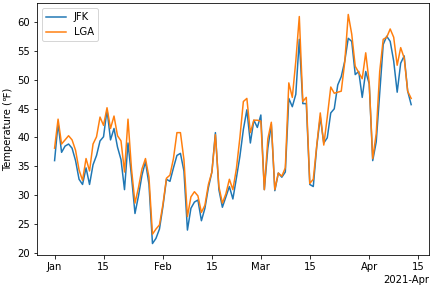
\includegraphics[width=1\textwidth]{figures/math/combined_artist.png}
    \caption{}
    \label{fig:math:combined}    
\end{subfigure}
\begin{subfigure}{.5\textwidth}
    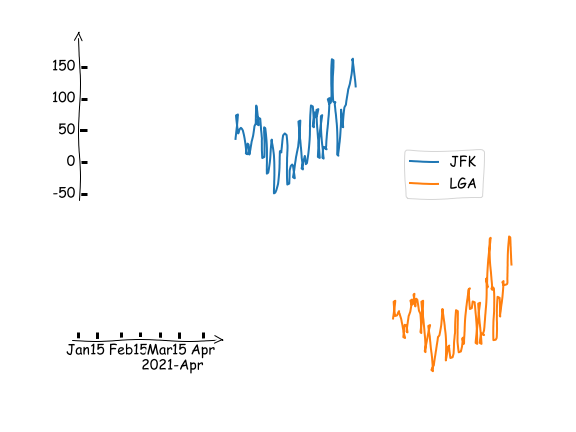
\includegraphics[width=1\textwidth]{figures/math/exploding_artist.png}
    \caption{}
    \label{fig:math:seperate}
\end{subfigure}
\caption{Each of the visual elements in \autoref{fig:math:seprate} is generated via a unique artist \vartist. In \autoref{fig:math:seperate}, they are added to the image independent of the other elements, creating an incoherant visualization. In \autoref{fig:math:combined}, these artists are composited before being added to the image. Disjoint union of \dtotal\ aligns the two timeseries with the x and y axis so all these elements use a shared coordinate system. A more complex composition dictates that the legend is connected to the \dtotal\ such that it must use the same color as the data it is identifying.}
\label{fig:artist_plus}
\end{figure}
We describe the constraints for compositing artists by defining addition operators. Given the family of artists $(\dtotal_i: i\in I)$ that are rendered to the same image, the + operator 
\begin{equation}
+ \coloneqq \underset{i\in I}{\sqcup} \dtotal_{i}
\end{equation}
defines a simple composition of artists. For example, the components in \autoref{fig:math:seperate} are each generated by different artists, and a visualization of solely the x axis is rarely all that useful. In \autoref{fig:math:seperate}, these artists are all added to the image independently of the other and therefore there are no constraints on how they are generated in conjunction with each other. In \autoref{fig:math:combined}, the data is joined via disjoint union; doing so aligns the components in \dfiber\ such the \vchannel\ to the same component in \vfiber\ targets the same coordinate system. When artists share a base space $\dbase_2 \hookrightarrow \dbase_1$, a composition operator can be defined such that the artists are acting on different components of the same section. This type of composition is important for visualizations where elements update together in a consistent way, such as multiple views \cite{alboRadarComparativeEvaluation2016a, hullmanKeeping2018} and brush-linked views\cite{beckerBrushingScatterplots1987,bujaInteractiveData1991}.


\subsubsection{Equivalance class of artists $\vartist^{\prime}$}
\label{sec:artist_equivalance}
\begin{figure}[H]
    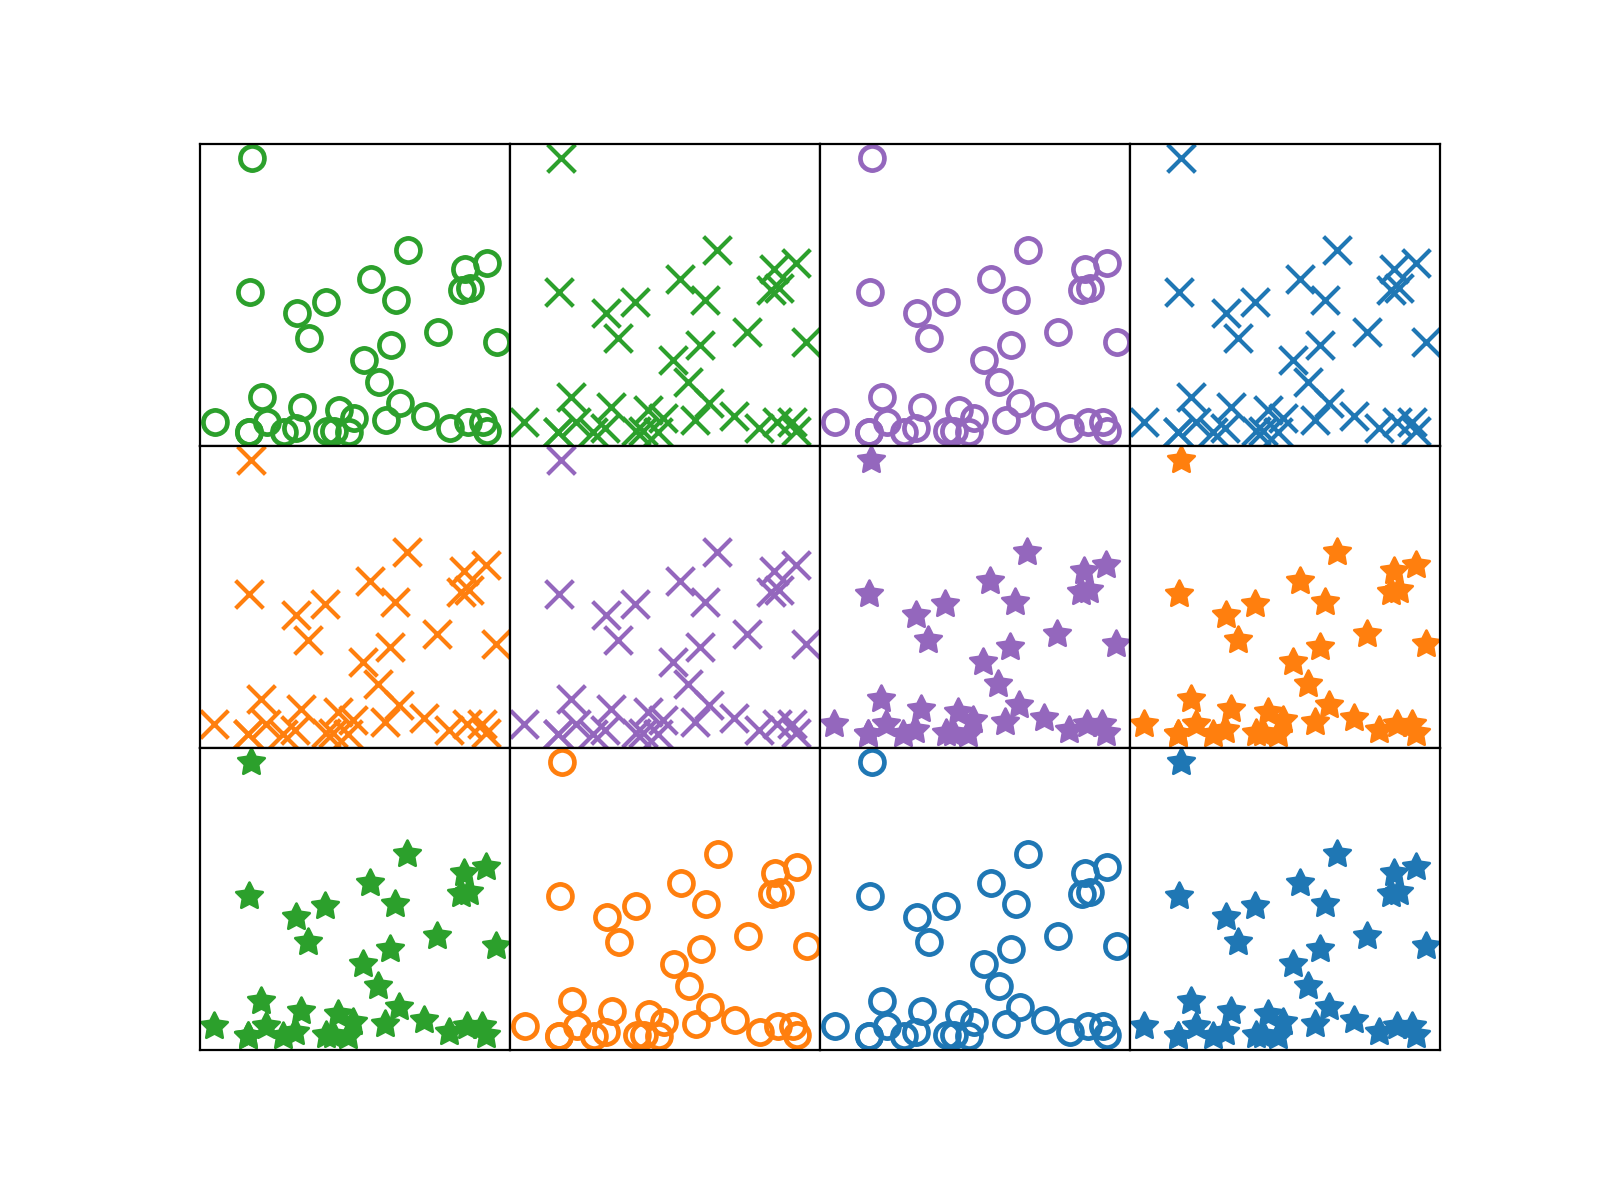
\includegraphics[width=1\textwidth]{figures/math/equivalent_artists.png}
   \caption{Each scatter plot is generated via a unique artist function $\vartist_{i}$, but they only differ in aesthetic styling. Therefore, these artists are all members of an equivalence class $\vartist_{i} \in \vartist{\prime}$}
    \label{fig:math:artist:equivalence}
\end{figure}
Representational invariance, as defined by Kindlmann and Scheidegger, is the notion that visualizations are equivalent if changing the visual representation, such as colors or shapes, does not change the meaning of the visualization\cite{kindlmannAlgebraicProcessVisualization2014}. We propose that visualizations are invariant if they are generated by artists that are members of an equivalence class 
\begin{equation*}
\{\vartist \in \vartist^{\prime}: \vartist_{1} \equiv \vartist_{2}\}
\label{eq:math:artist:aprime}
\end{equation*}
For example, every scatter plot in \autoref{fig:math:artist:equivalence} is a scatter of the same datasets mapped to the \textit{x position} and \textit{y position} in the same way. The scatter plots only differ in the choice of constant visual literals, differing in color and marker shape. Each scatter is generated by an artist $\vartist_{i}$, and every scatter is generated by a member of the equivalence class $\vartist_{i} \in \vartist{\prime}$. Since it is impractical to implement a new artist for every single graphic, the equivalance class provides a way to evaluate an implementation of a generalized artist. Given equivalent, but no necessarily identical, \vchannel, \vmark, and \vindex, two artists are equivalent. This criteria also allows for comparing artists across libraries. 
\end{document}